\documentclass[twoside,twocolumn]{article}


% \usepackage[sc]{mathpazo} % Use the Palatino font
\usepackage[T1]{fontenc} % Use 8-bit encoding that has 256 glyphs
\linespread{1.05} % Line spacing - Palatino needs more space between lines
\usepackage{microtype} % Slightly tweak font spacing for aesthetics


\usepackage[english]{babel} % Language hyphenation and typographical rules

\usepackage[hmarginratio=1:1,top=32mm,columnsep=20pt, margin=2cm]{geometry} % Document margins
\usepackage[small,labelfont=bf,up,textfont=it,up]{caption} % Custom captions under/above floats in tables or figures
\usepackage{booktabs} % Horizontal rules in tables

\usepackage{enumitem} % Customized lists
\setlist[itemize]{noitemsep} % Make itemize lists more compact

\usepackage{abstract} % Allows abstract customization
\renewcommand{\abstractnamefont}{\normalfont\bfseries} % Set the "Abstract" text to bold
% \renewcommand{\abstracttextfont}{\normalfont\small\itshape} % Set the abstract itself to small italic text

\usepackage{titlesec} % Allows customization of titles
\titleformat{\section}[block]{\large\scshape\centering}{\thesection.}{1em}{} % Change the look of the section titles
\titleformat{\subsection}[block]{\large}{\thesubsection.}{1em}{} % Change the look of the section titles

\usepackage{titling} % Customizing the title section

\usepackage{cite}
% \addbibresource{report.bib}
\usepackage{siunitx}
\sisetup{
    separate-uncertainty = true,
    % multi-part-units = single
    }
\DeclareSIUnit \parsec {pc}

\usepackage{bm}
\usepackage{braket}
    
\usepackage{graphicx}
\usepackage{array}
\newcolumntype{P}[1]{>{\raggedright\arraybackslash}p{#1}}
\usepackage{url}
\usepackage{amsmath}

\usepackage{listings}
\lstset{showstringspaces=false, language=Python, breaklines=true, basicstyle=\small}

%----------------------------------------------------------------------------------------
%	TITLE SECTION
%----------------------------------------------------------------------------------------

\setlength{\droptitle}{-4\baselineskip} % Move the title up

\pretitle{\begin{center}\Huge\bfseries} % Article title formatting
\posttitle{\end{center}} % Article title closing formatting
\title{Tidal Tails and Interacting Galaxies} % Article title
\author{%
    \normalsize University of Cambridge \\ % Your institution
    }
\date{
    \today \\
} % Leave empty to omit a date

\renewcommand{\maketitlehookd}{%

\begin{abstract}
    A tidal tail is a long, thin region of stars and interstellar dust extending from a galaxy, and is a result of tidal gravitational forces between interacting galaxies. A simple N-body simulation of two interacting galaxies was performed where specifically, a star-less perturbing galaxy with initial conditions of a parabolic orbit was introduced to a central galaxy with circularly orbiting stars. The simulation showed that the tidal tail was created from the outer orbiting stars of the central galaxy through a prograde encounter between the perturbing galaxy and the central galaxy. Quantitative results, including the fraction of stars disturbed from their initial orbits and the median distance of the stars from the central galaxy, were obtained for different characteristics and initial conditions of the perturbing galaxy. Varying the distance of closest approach of the two galaxies showed a smaller distance of closest approach leads to a larger proportion of disturbed stars and a larger median distance between the stars and the central galaxy. Changing the mass of the perturbing galaxy demonstrated that the heavier the perturbing galaxy, more stars were stripped away and ended up further away from the central galaxy. [Word count: 2932]

    
\end{abstract}
}


\begin{document}

\maketitle

\section{Introduction}
    Tidal tails are long, thin, and often curved regions of stars and interstellar debris extending from a galaxy, and are a result of the strong tidal gravitational forces of interacting galaxies. Tidal tails are often a useful feature in the study and characterisation of the evolution of galactic phenomena, which includes galaxy mergers and the formation of tidal dwarf galaxies \cite{alavi}. A well-known example of tidal tails is the Antennae Galaxies -- a pair of galaxies currently undergoing galactic collision. The system's pair of prominent tidal tails extend from the top of the two galaxies and is what gives its characteristic insect-like outline, as seen in Figure \ref{figure:antennae}. The Tadpole Galaxy provides another good example of tidal tails, where its long tidal tail of approximately \SI{86}{\kilo\parsec} has been attributed to a merger with a smaller galaxy in the past \cite{tadpole}. An image of the Tadpole Galaxy is provided in Figure \ref{figure:antennae}.
    
    \begin{figure}
        \centering
        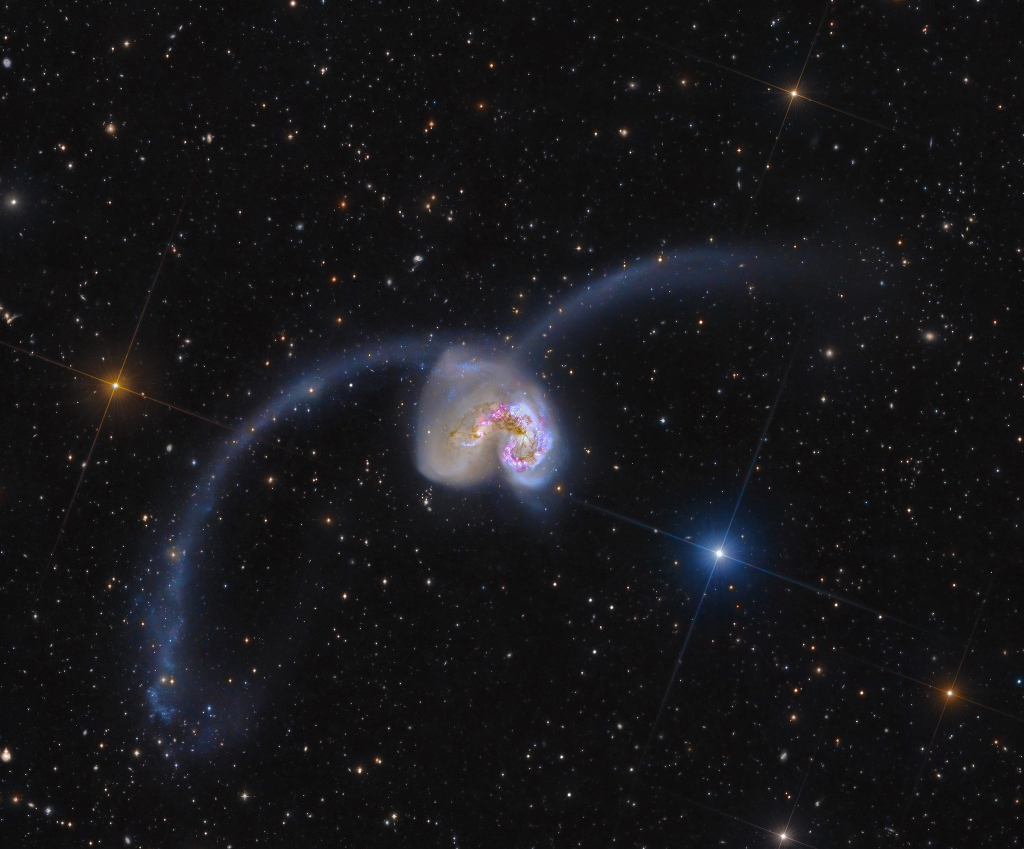
\includegraphics[width=0.9\linewidth]{images/antennae.png}

        \vspace{0.2cm}
        
        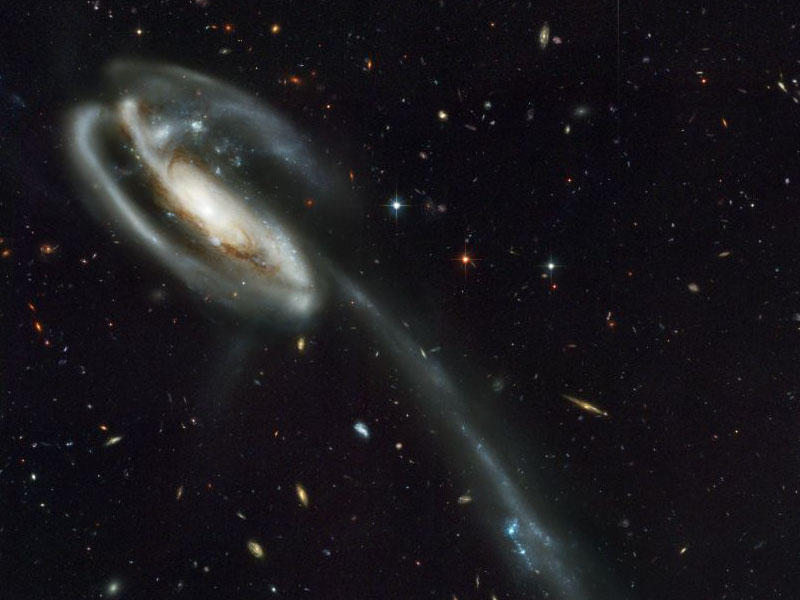
\includegraphics[width=0.9\linewidth]{images/tadpole_tail.png}
        \caption{Top image: The Antennae Galaxies. A pair of prominent tidal tails can be seen extending from both sides of the system. Bottom image: Tadpole Galaxy. Its characteristic long tidal tail can be seen extending from the core of the galaxy.}
        \label{figure:antennae}
        
    \end{figure}

    The formation of tidal tails is a difficult phenomenon to describe analytically, thus computer simulations have come in handy to provide possible explanations for its formation. In one of the first simulations of the interaction between two galaxies by Toomre and Toomre in 1972 \cite{toomre}, they found that tidal tails were primarily formed through prograde encounters between the 'central' and perturbing galaxy, where both the stars in the central galaxy and the perturbing galaxy are orbiting in the same direction. Toomre and Toomre used the restricted three-body equations of motion, alongside the fourth-order Runge-Kutta method in order to simulate the interaction. A few years later, Keenan and Innanen investigated the same effects using numerical methods, and came to the same conclusion as Toomre and Toomre \cite{keenan}. Their studies were able to accurately reconstruct the appearance and outer outlines of a number of galactic systems, including Arp 295, M51 + NGC 5195, NGC 4676 and the Antennae Galaxies.

    Just like in the simulations mentioned above, the aim of this investigation is to run a simple N-body simulation of two interacting galaxies, which shall be called the \emph{central} and \emph{perturbing} galaxies. The central galaxy will contain test particles, which represent the stars and interstellar dust, orbiting around a central heavy mass at multiple radii. Given that the masses of stars are negligible compared to the central mass of a galaxy, the test particles' masses can and will be assumed to be zero in this investigation. The perturbing galaxy will be introduced with the initial conditions of a parabolic orbit, and the effects of this perturbing galaxy will be observed.


\section{Analysis}    

    The primary concern of this investigation is the choice of the N-body simulation method. As stated by Toomre and Toomre in their paper form 1972, there are two simple methods that can be used for such simulations -- the timestep method, and the integration of the restricted three-body equations of motion using the fourth-order Runge-Kutta method. There are also more modern and sophisticated techniques, such as tree methods (Barnes-Hut) and particle mesh methods, which reduces the runtime of the such simulations. These methods were not considered here due to their complexity, as well as the small scale of this investigation not requiring high efficiency. The timestep and restricted three-body methods for a single test particle are outlined below:
    \vspace{0.2cm}

    \noindent \textbf{Timestep method}
    \begin{enumerate}
        \item Provide the initial position $(x_0, y_0)$ and velocity $(v_{x,0}, v_{y,0})$ of the test particle.
        \item Calculate the forces acting on the test particle, resolving them in each axis direction. Working in two dimensions, the gravitational acceleration acting in each axis direction as a result of a massive object is
        \begin{equation}
            a_{x} = \frac{GM(x - X)}{r^3}, \ \ a_{y} = \frac{GM(y - Y)}{r^3}
            \label{eqn:acceleration}
        \end{equation}
        where $G$ is the gravitational constant, $M$ is the mass of the massive object, $(x, y)$ is the position of the test particle, $(X, Y)$ is the position of the massive object and $r = \sqrt{(x - X)^2 + (y - Y)^2}$. 
        \item Let $\delta t$ be a small timestep. The velocity, as a result of the gravitational acceleration, is
        \begin{equation}
            v_x = v_{x,0} + a_{x} \delta t, \ \ v_y = v_{y,0} + a_{y} \delta t
        \end{equation}
        and the position is
        \begin{equation}
            x = x_0 + v_x \delta t, \ \ y = y_0 + v_y \delta t
        \end{equation}
        \item Repeat these steps until the end time is reached.
    \end{enumerate}
    \vspace{0.2cm}

    \noindent \textbf{Restricted three-body method}
    \begin{enumerate}
        \item For the three-body system, the equation of motion is given as \cite{three_body}
        \begin{equation}
            \begin{split}
                &a_{x} = - \frac{GM_1(x - X_1)}{r_1^3} - \frac{GM_2(x - X_2)}{r_2^3} \\
                &a_{y} = - \frac{GM_1(y - Y_1)}{r_1^3} - \frac{GM_2(y - Y_2)}{r_2^3},
            \end{split}
        \end{equation}
        where $M_{1,2}$ are the masses of the massive objects, $(X_{1, 2}, Y_{1, 2})$ are the positions of the massive objects and $r_{1, 2}$ are the distances between the test particle and the massive objects. 
        \item Two first order ODEs in each axis direction are obtained from the equation of motion. The fourth-order Runge-Kutta method is then used here to integrate the first order ODEs for each test particle.
        \item The motion of the test particle is then known based off the motion of the two massive interacting bodies.
    \end{enumerate}
    
    \begin{figure}
        \centering
        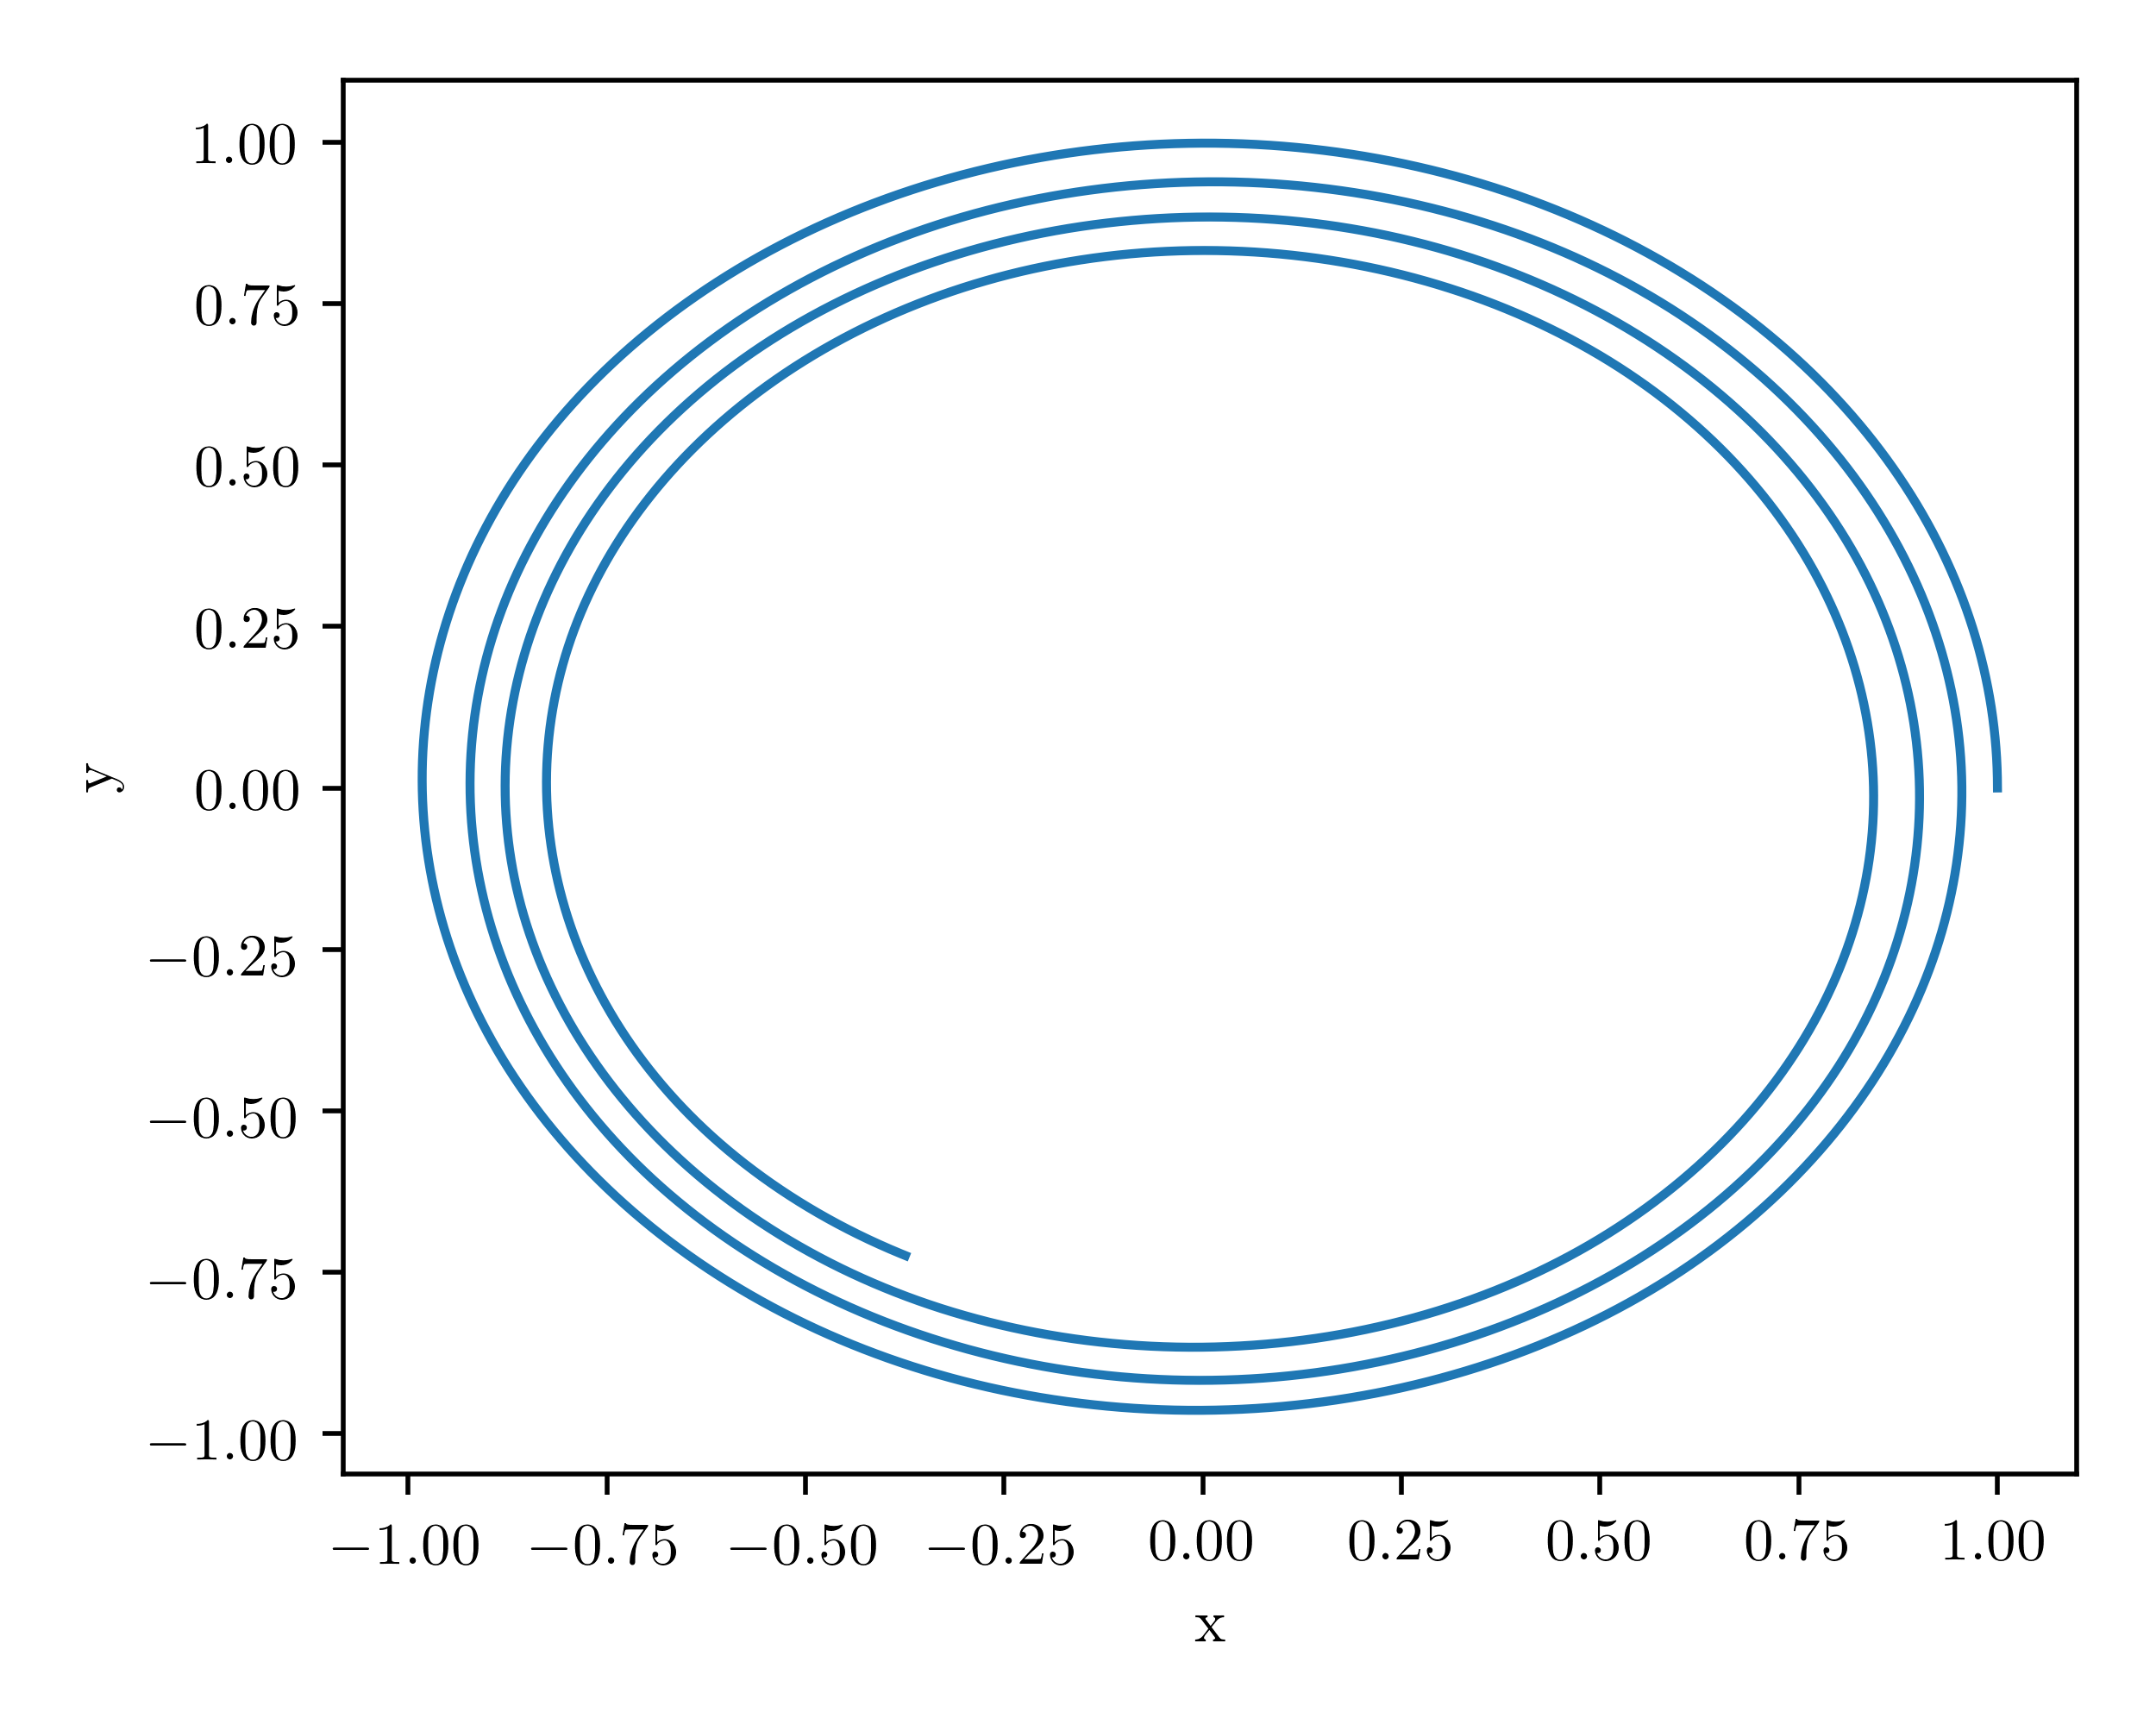
\includegraphics[width=\linewidth]{images/RK45.png}
        \caption{With the central mass positioned at $(0, 0)$ and the test particle having an initial velocity $v = \sqrt{GM/r}$, the path of the test particle spirals inward when the fourth-order Runge-Kutta method is used to integrate its equation of motion.}
        \label{figure:RK45}
        
    \end{figure}

    In order to determine the preferred technique, these two methods were tested on a simple two-body system consisting of a large mass and a circularly orbiting test particle. This small experiment showed that the Runge-Kutta method lost its accuracy quickly for orbiting systems such as this one, where the path of the test particle was found to spiral inward, as shown in Figure \ref{figure:RK45}. The timestep method, despite being more inefficient, proved to be more accurate for such a system. Thus, the timestep method was the method of choice for this investigation into the effects of interacting galaxies.

    Another key computational aspect in this investigation was the use and storage of the calculated particle trajectories from the simulation. Knowing that the simulation will contain many test particles, potentially $>1000$ particles, it was important to keep in mind that a good system to store and read the calculated data was required. Such a system would most likely require to be able to create and read multiple large \texttt{.csv} files for the experiments that will be performed. 
    

\section{Implementation}
    \label{section:implementation}

    This N-body simulation contained 1200 test particles of zero mass orbiting circularly around the central galaxy. To be more detailed, there were 120, 180, 240, 300 and 360 particles orbiting at a radius of 2, 3, 4, 5 and 6 units respectively. The perturbing galaxy contained no test particles (to simplify the problem), and it had the initial conditions of a parabolic orbit about the central galaxy. The test particles experienced the gravitational forces of both massive galaxies, whilst both galaxies experienced the gravitational force from each another. Note that the gravitational constant $G = 1$ was used in this simulation, and units were arbitrary and generally disregarded here.

    A few experiments were performed with this simulation, and they are given below:
    \begin{itemize}
        \item comparing prograde and retrograde encounters,
        \item varying the mass of the perturbing galaxy,
        \item and varying the distance of closest approach of the perturbing galaxy.
    \end{itemize}
    Two quantitative metrics were used here to quantify the two latter experiments -- the fraction of test particles disturbed from their initial orbits, and the median distance of the test particles from the central galaxy. Here, the term "disturbed" was arbitrarily defined as when the test particle deviates from its original orbiting radius by $>0.5$. The choice of using the median instead of the average was due to the possibility of stray test particles being 'shot' very far out. More details of this will be given in \S \ref{section:error}.

    \subsection{Physics}
        \label{section:physics}

        In order for test particles to orbit around the central galaxy in a stable circular fashion, suitable initial velocities were required. Equating the centripetal force and the gravitational force, a test particle required its velocity $\bm{v}$ to have a magnitude $\lvert\bm{v}\lvert = \sqrt{GM/r}$, travelling perpendicular to the radial direction. The velocities in the $x$ and $y$ direction could then be written as $v_x = - \lvert\bm{v}\lvert \sin{\theta}$ and $v_y = \lvert\bm{v}\lvert \cos{\theta}$, where $\theta$ is the angle between the positive x-axis and the position vector of the test particle relative to the central galaxy. Note that the test particles were initialised such that they orbit the central galaxy in the anti-clockwise direction.

        As mentioned above, the perturbing galaxy is initially in a parabolic orbit. A parabolic orbit has the characteristic of the system having zero net energy, where the kinetic energy is balanced with the gravitational potential energy. This can be shown as
        \begin{equation}
            E = 0 = \frac{mv^2}{2} - \frac{GMm}{r}
        \end{equation}
        where $M$ is the mass of the central galaxy, $m$ is the mass of the perturbing galaxy, $v$ is the velocity of the orbiting mass and $r$ is the distance between the central and orbiting masses. Solving this leads to a velocity with magnitude $v = \sqrt{2GM/r}$. 
        
        The trajectory of a parabolic orbit is given by \cite{lecture}
        \begin{equation}
            y^2 = 4r_{min}^2 - 4r_{min}x,
        \end{equation}
        where $r_{min}$ is the minimum distance of approach of the orbiting mass. The initial velocities of the perturbing galaxy in the $x$ and $y$ direction can then be determined using $v^2 = v_x^2 + v_y^2$ and the derivative of the trajectory $y' = dy/dx = v_x/v_y$. Combining these equations give
        \begin{equation}
            v_y = \pm \frac{y'\lvert\bm{v}\lvert}{\sqrt{1 + y'^2}}, \ v_x = \frac{v_y}{y'}.
        \end{equation}
        It was important to keep track of the signs here since the perturbing galaxy could be introduced either prograde or retrograde with respect to the test particles orbiting in the anti-clockwise direction.
    
\begin{figure*}
    \centering
    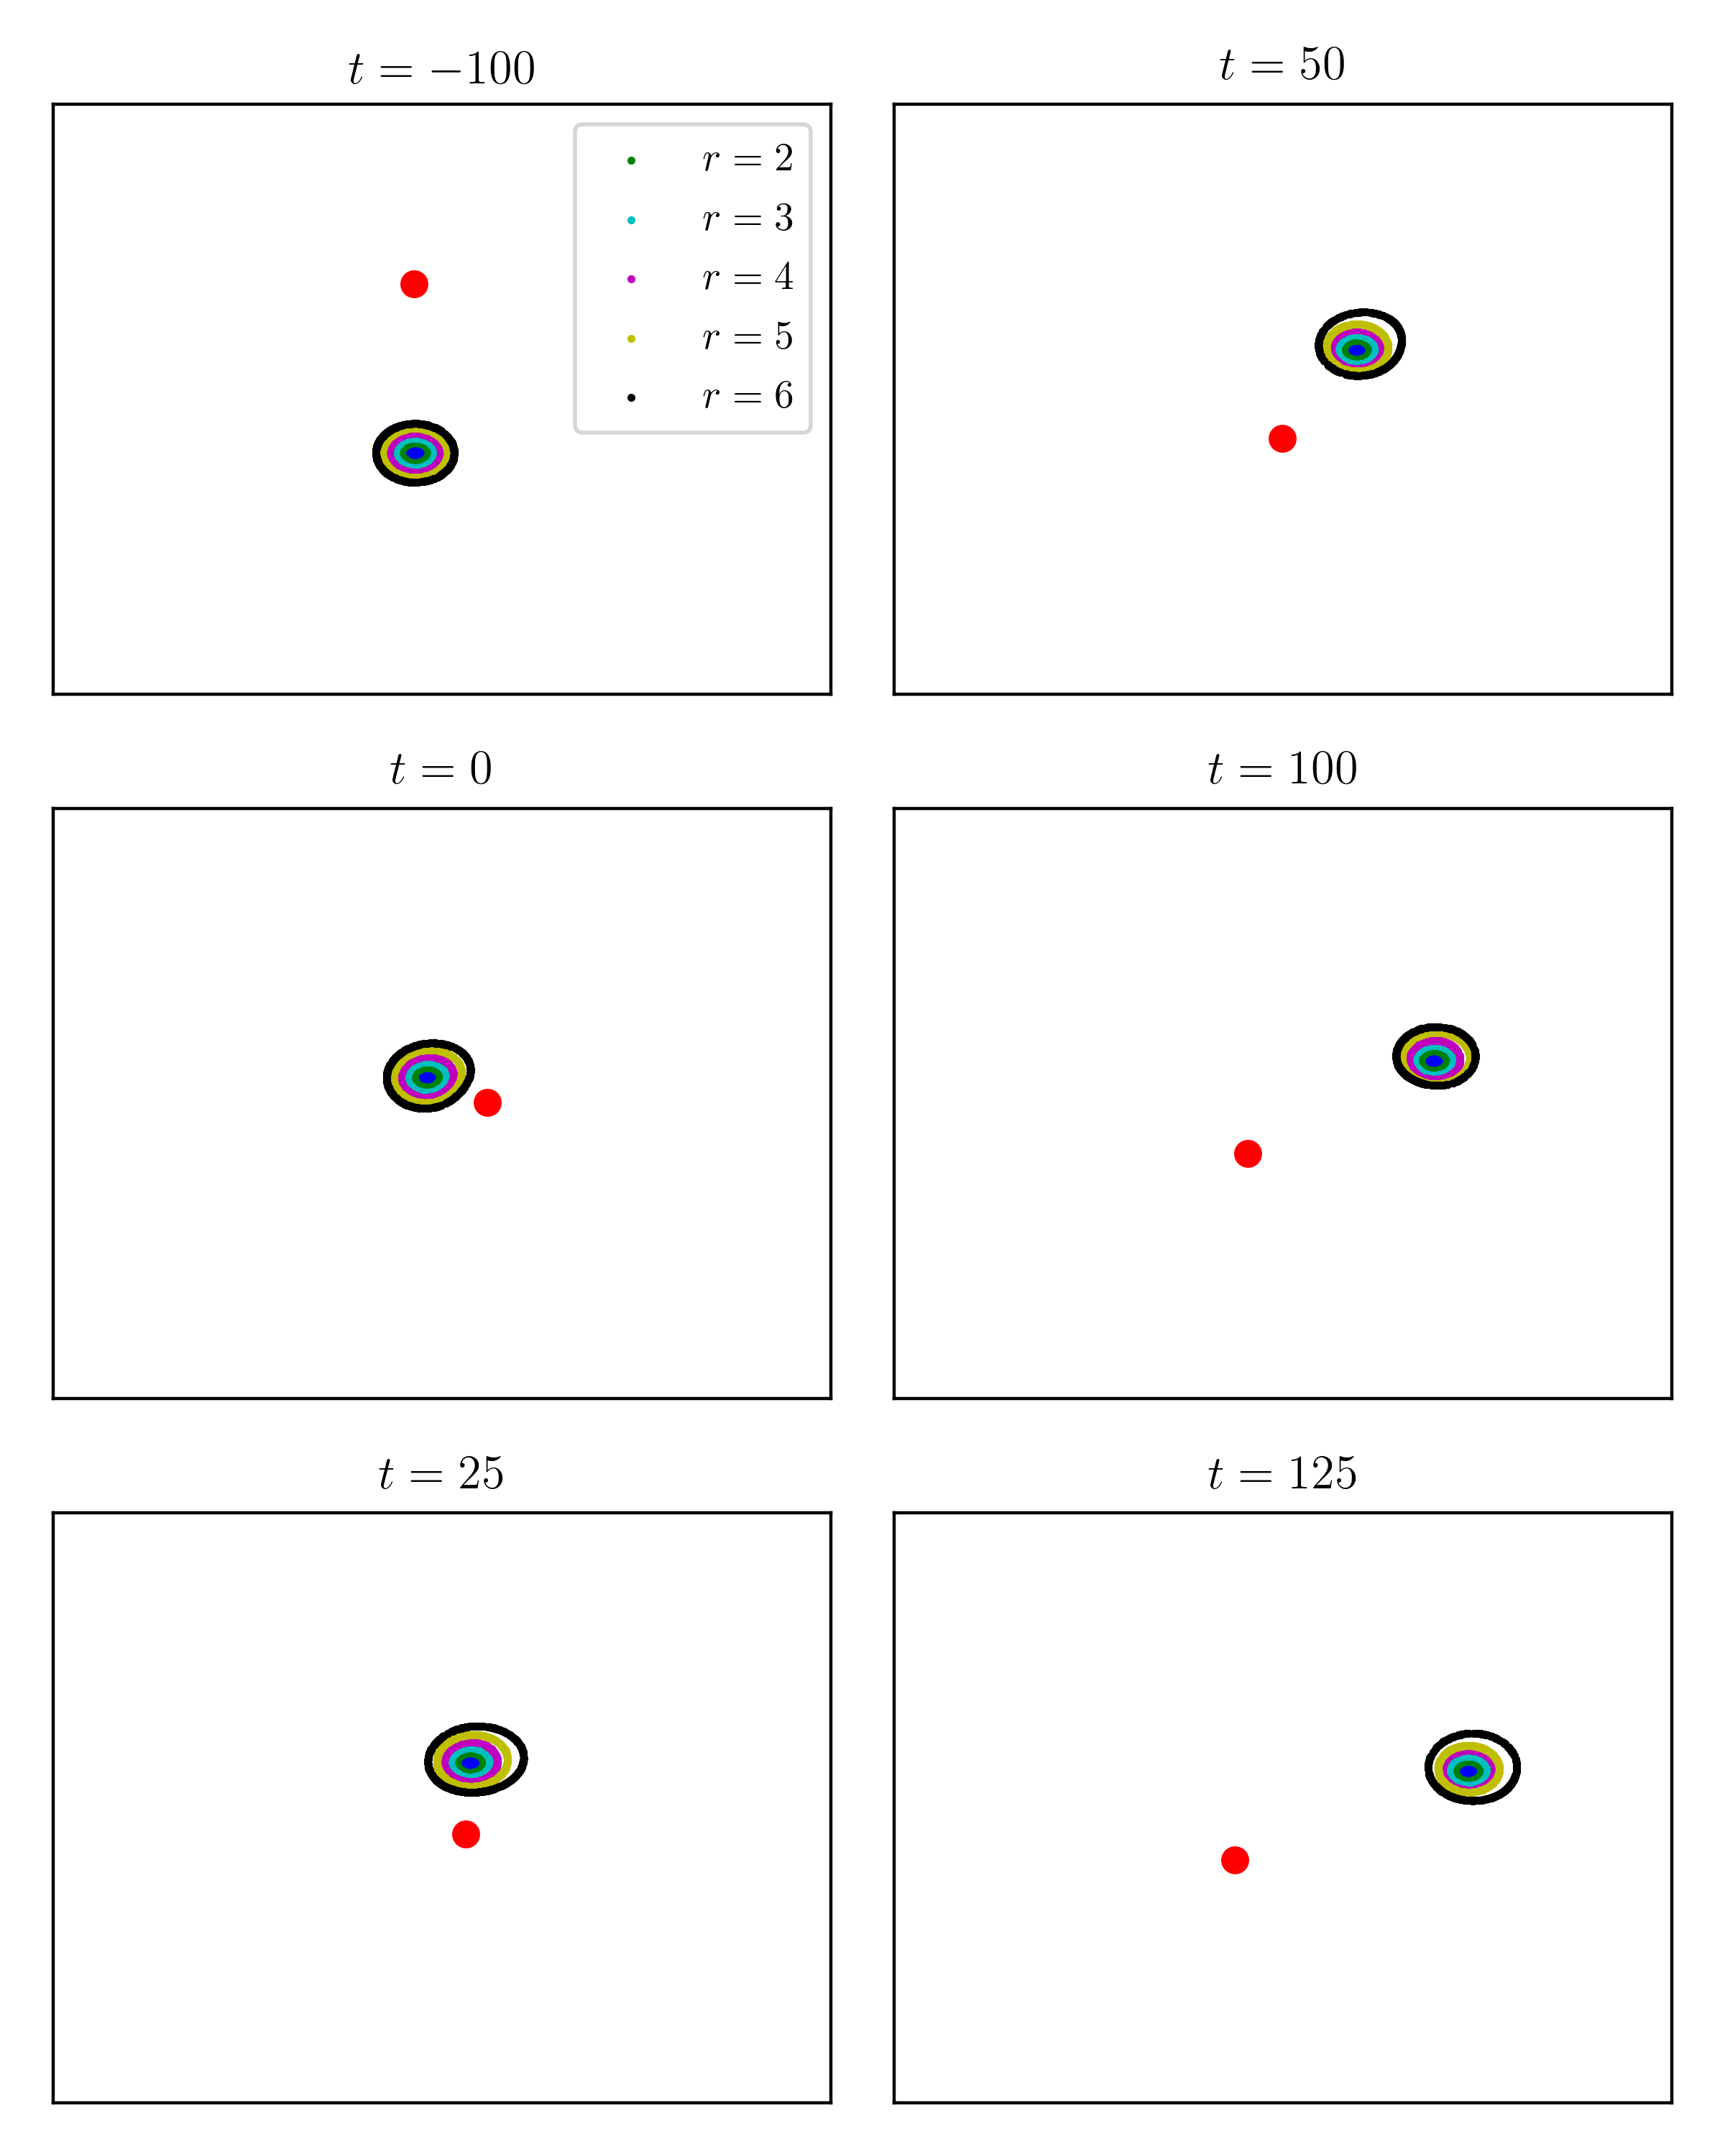
\includegraphics[width=\linewidth]{images/clockwise_positions.png}
    \caption{A time evolution of the retrograde encounter between the two galaxies for variables \texttt{r\_min = 20} and \texttt{mass = 1}. Notice that none of the stars are thrown out of orbit, however the outer orbiting stars seem to have its orbit destabilised.}
    \label{figure:retrograde}
\end{figure*}

\begin{figure*}
    \centering
    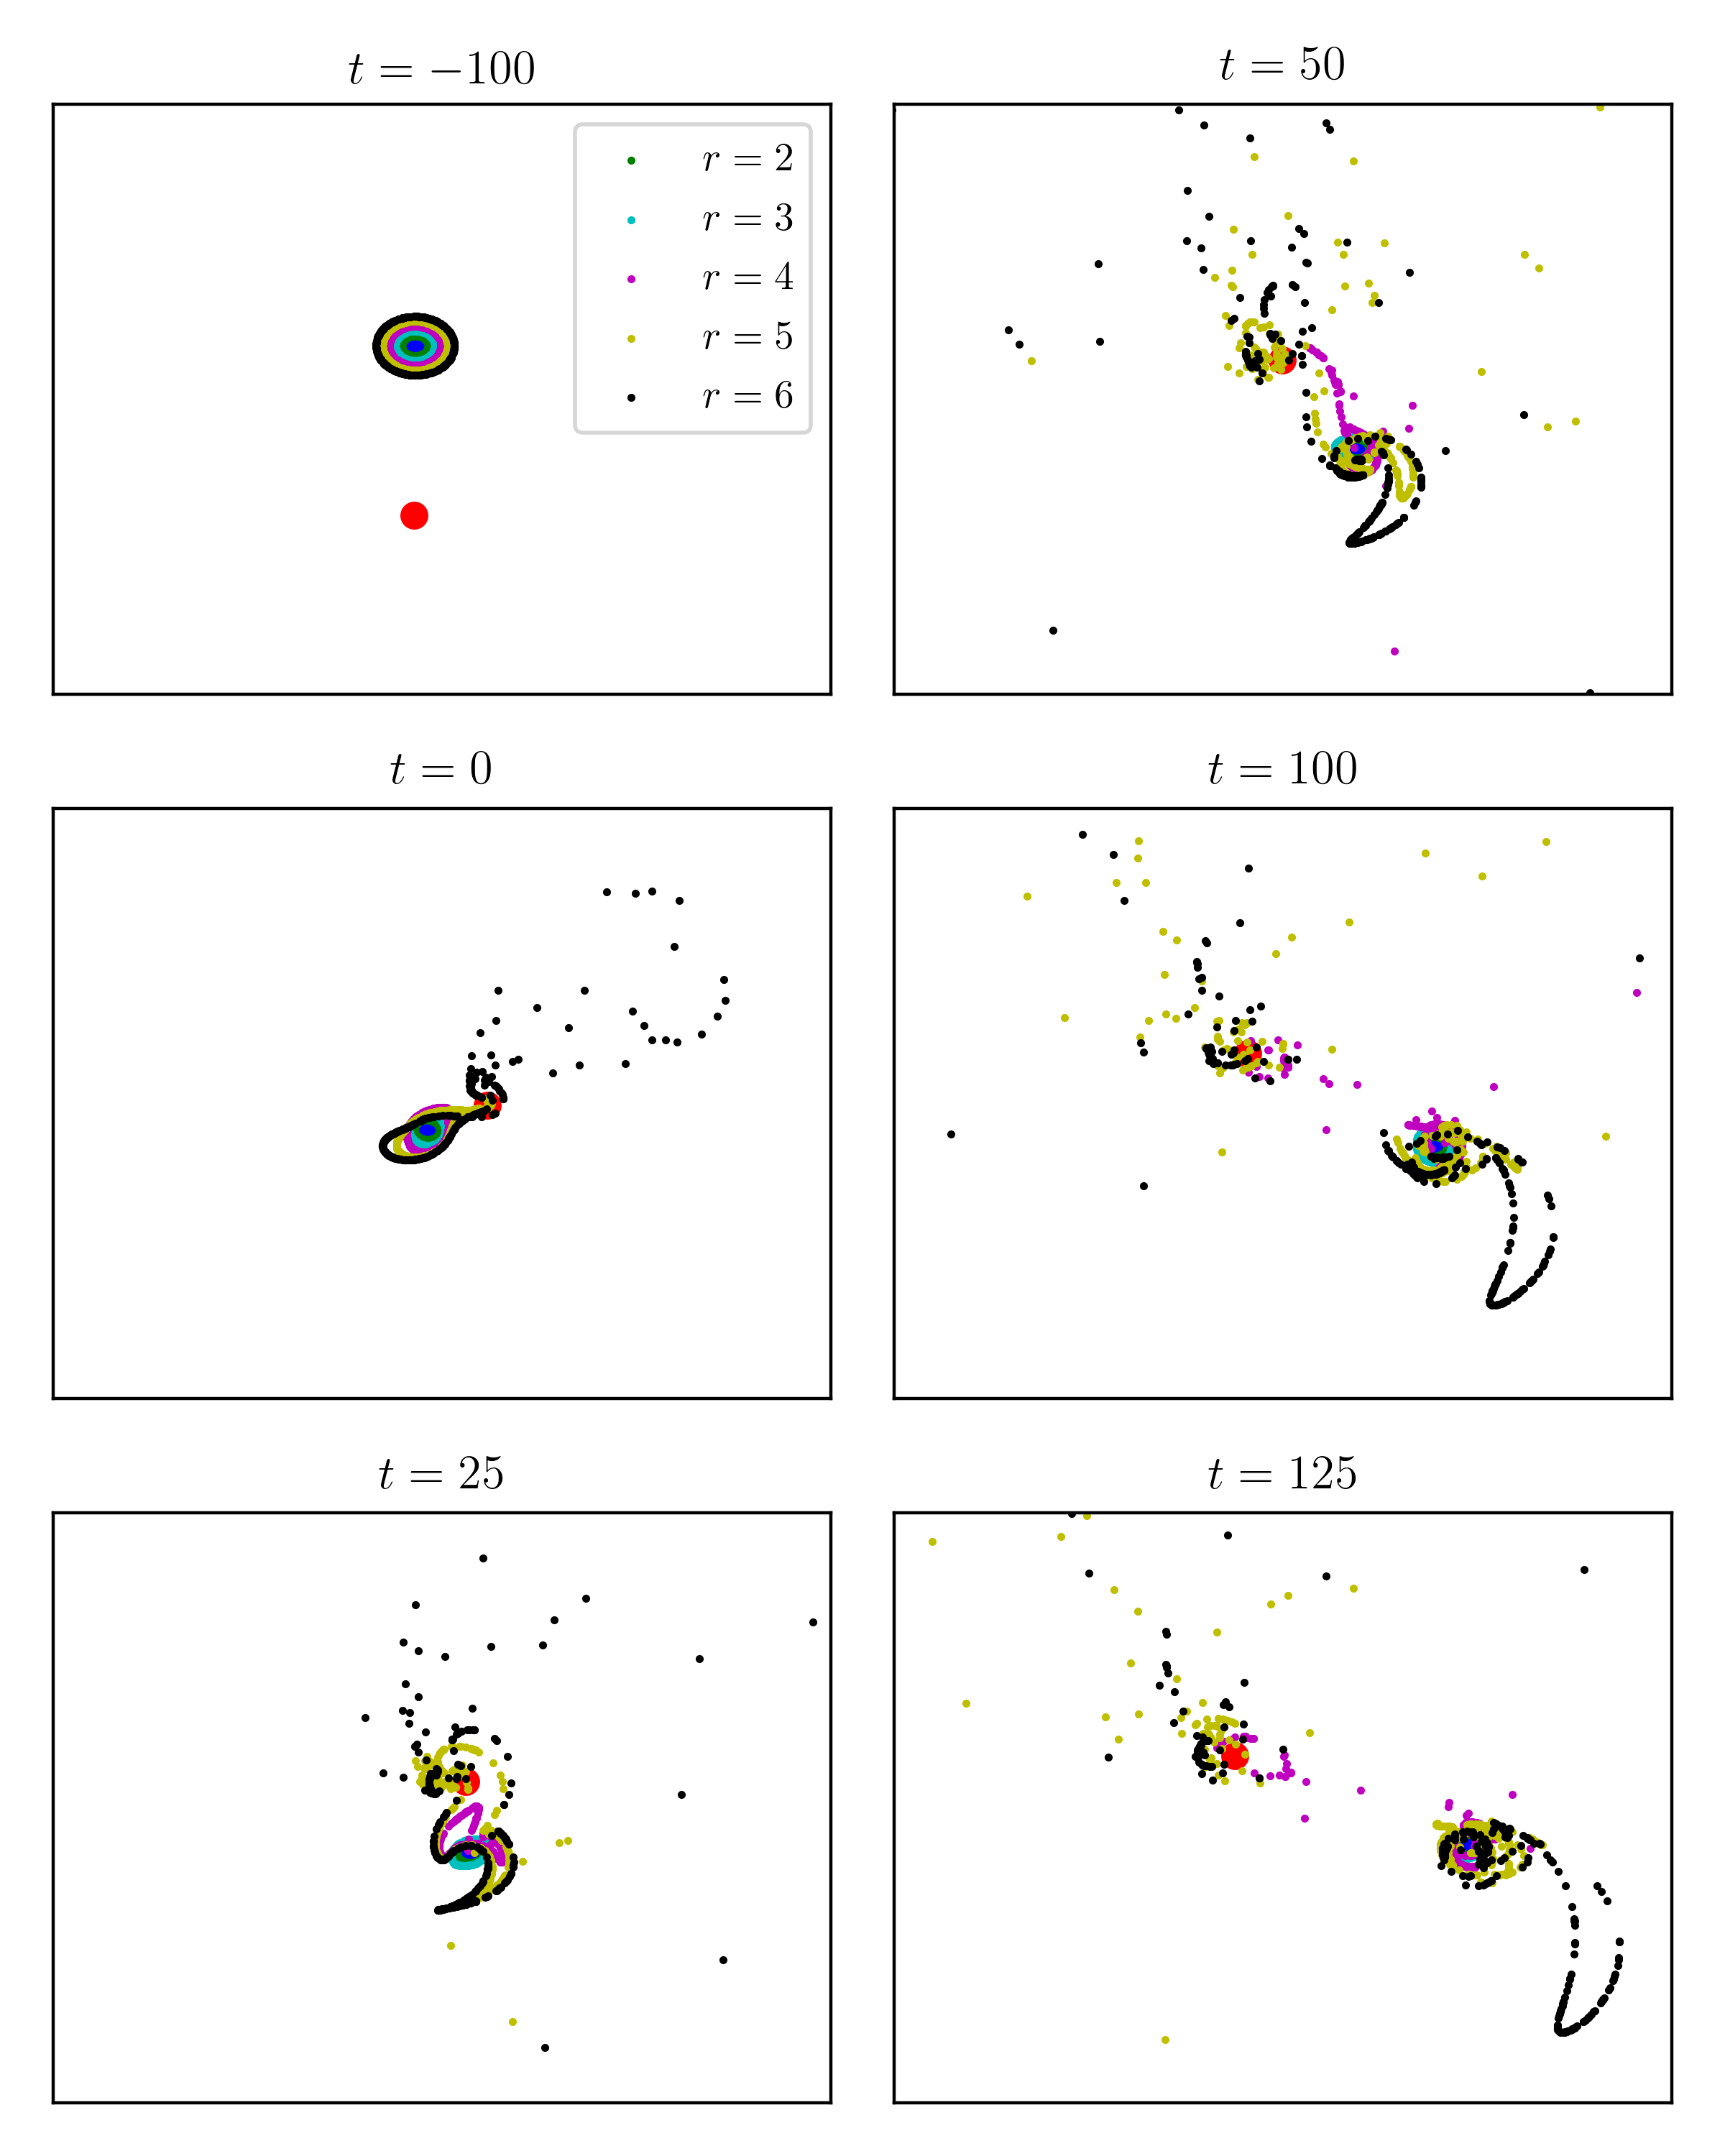
\includegraphics[width=\linewidth]{images/anticlockwise_positions.png}
    \caption{A time evolution of the prograde encounter between the two galaxies for variables \texttt{r\_min = 20} and \texttt{mass = 1}. The final two snapshots of the encounter show the development of a tidal tail made up of stars from the outer orbits of the central galaxy.}
    \label{figure:prograde}
\end{figure*} 
        
    \subsection{Code}
        A \texttt{Body} class was created to represent both the massive galaxies and test particles. This class contains two important functions, \texttt{set\_gforce} and \texttt{update\_speed\_position}, which obtains the resultant forces acting on the body and updates the body's speed and position respectively. This class is housed in the \texttt{core.py} file. This file also contains two other important functions -- \texttt{initialise\_moving\_body} which initialises the perturbing galaxy in its parabolic orbit with the velocities from \S \ref{section:physics}, and \texttt{initialise\_test\_particles} which initialises all the test particles at random angles around the central galaxy.
        
        The \texttt{simulation.py} contains the script which runs the simulation and writes the position data from the simulation into suitably named files. A small timestep of \texttt{dt = 0.1} was used to iterate through from \texttt{t = 0} to \texttt{t = 700}, where the positions and velocities of the galaxies and test particles were updated at each iteration. This file, alongside the \texttt{core.py} file, allows multiple runs of the simulation for different variables (distance of closest approach \texttt{r\_min}, mass of perturbing galaxy \texttt{mass}) to be performed consecutively.
        
        The \texttt{animation.py} and \texttt{get\_quantitative.py} files were used to read the \texttt{.csv} files, albeit with different functions. The former was used to create a simple animation of the interaction with \texttt{matplotlib}, and the latter was used to extract the quantitative metrics from the data produced from the simulation.

        The code in these files can be found in the Appendix.

        
        
    \subsection{Performance}
    
    Given the large number of test particles, the simulation was expected to take some time to run, especially given the limitations of the hardware of a laptop. Particular attention was given to using Python's list comprehension rather than using \texttt{for} loops in order to improve the runtime of the program. One run of the simulation took on average around \SI{90}{\second} on a laptop with an i5 two core processor.
    
    When it came to reading the large \texttt{.csv} files, the main bottleneck was loading the position data from the file into the laptop's memory. Two known built-in methods that does this job are \texttt{numpy}'s \texttt{loadtxt} and \texttt{pandas}'s \texttt{read\_csv} methods. It was found that \texttt{pandas.read\_csv} method was significantly faster than \texttt{numpy.loadtxt}, where \texttt{pandas.read\_csv} took around \SI{9}{\second} whereas \texttt{numpy.loadtxt} took around \SI{22}{\second}. Thus, the \texttt{pandas} method was chosen to be used here.
        
        
\section{Results and Discussion}   

    \subsection{Prograde and Retrograde Encounters}

        Figure \ref{figure:retrograde} and \ref{figure:prograde} show the retrograde and prograde encounters of the two galaxies respectively. Here, the distance of closest approach \texttt{r\_min} was set to 20 units and the mass of the perturbing galaxy \texttt{mass} was set to 1 unit. The \texttt{t = 0} snapshot was set to the frame where the distance between the two galaxies was at a minimum. Multiple runs of the same simulation were performed, and very similar results were obtained from them. The figures show a clear agreement between the results of this simulation and those performed by Toomre and Toomre, where the prograde encounter was shown to have a significantly more disruptive effect than the retrograde encounter. 
        
        In the retrograde encounter, there was a noticeable destabilisation of the outermost circular orbit in the $t = 25, 50, 100, 125$ snapshots. However, the outermost stars remained in orbit, albeit not circular, around the central galaxy. This mild effect can possibly be attributed to weak tidal effects from the perturbing galaxy, where the test particles nearest to the perturbing galaxy moved in a relatively antiparallel direction to the velocity of the perturbing galaxy.
        
        In the prograde encounter, strong tidal effects, arising from the similarity in the direction of the velocities of the test particles and perturbing galaxy, tore apart the outer stars with an orbiting radius of 4, 5 and 6 units. The formation of the tidal tail, which was made up of the outermost stars (radius of 6 units), seen in the bottom right corner of the $t = 100, 125$ snapshots was the most noticeable effect of such strong tidal forces. A large proportion of the outer stars were taken away by the perturbing galaxy, where these stars form new orbits around the perturbing galaxy. A considerable amount of stars were also seem to have been flung away from both galaxies in a seemingly random distribution.

    \subsection{Varying Initial Conditions of Perturbing Galaxy}

        \begin{figure}
            \centering
            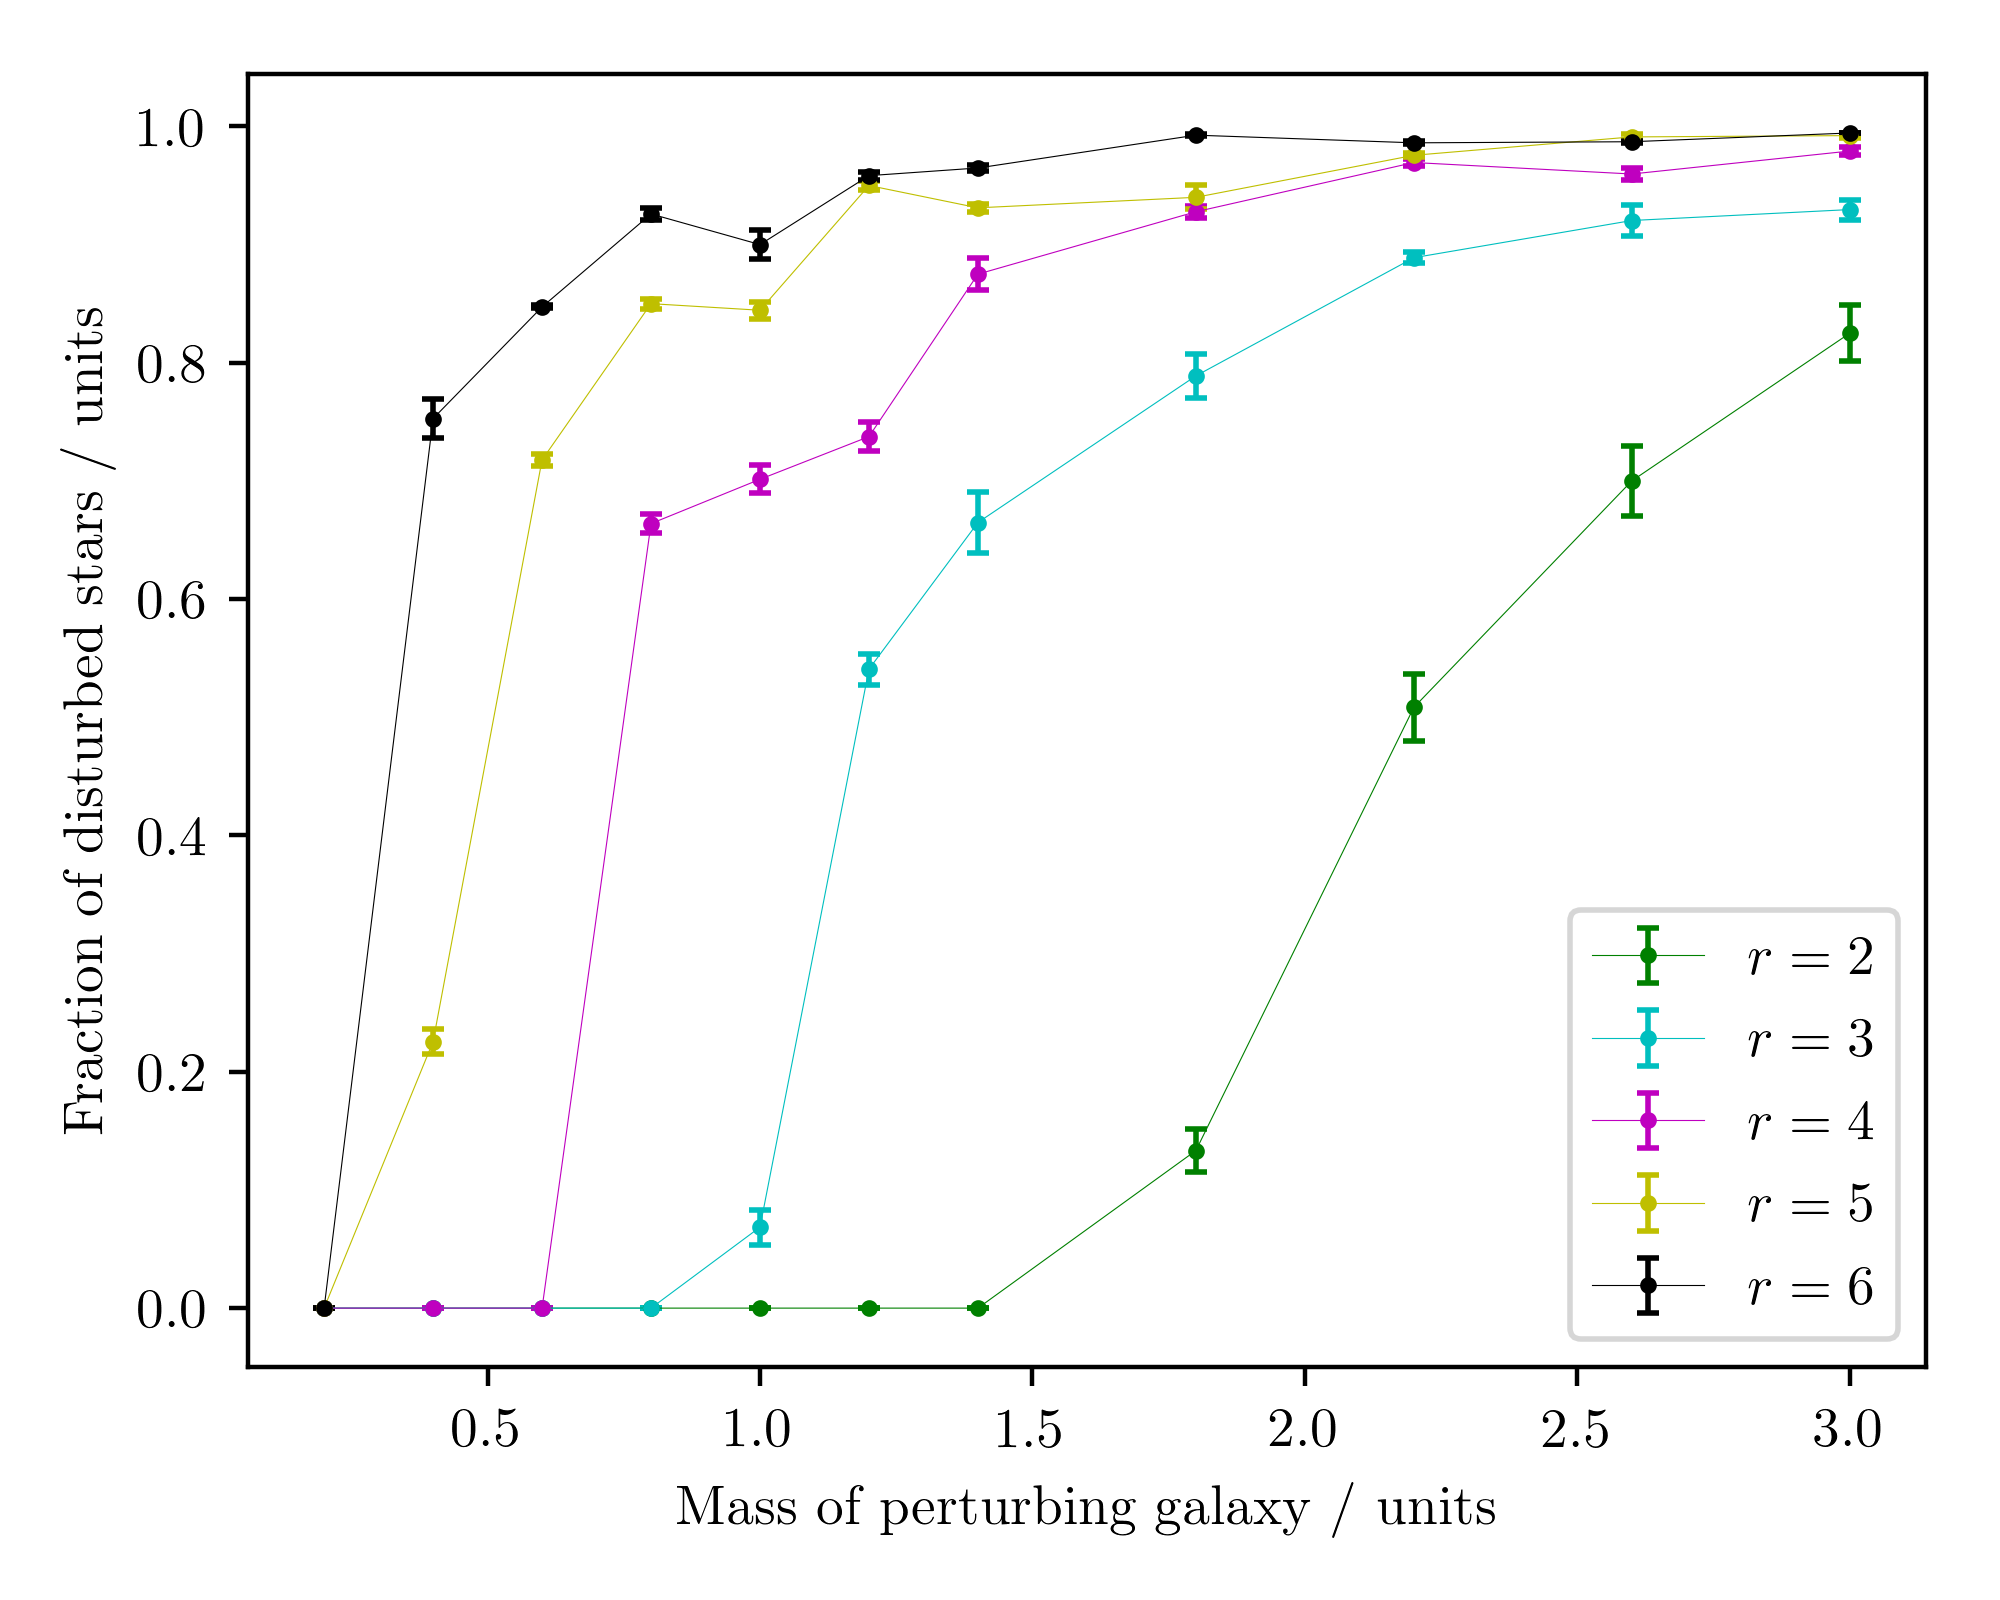
\includegraphics[width=\linewidth]{images/plot_fraction_mass.png}
            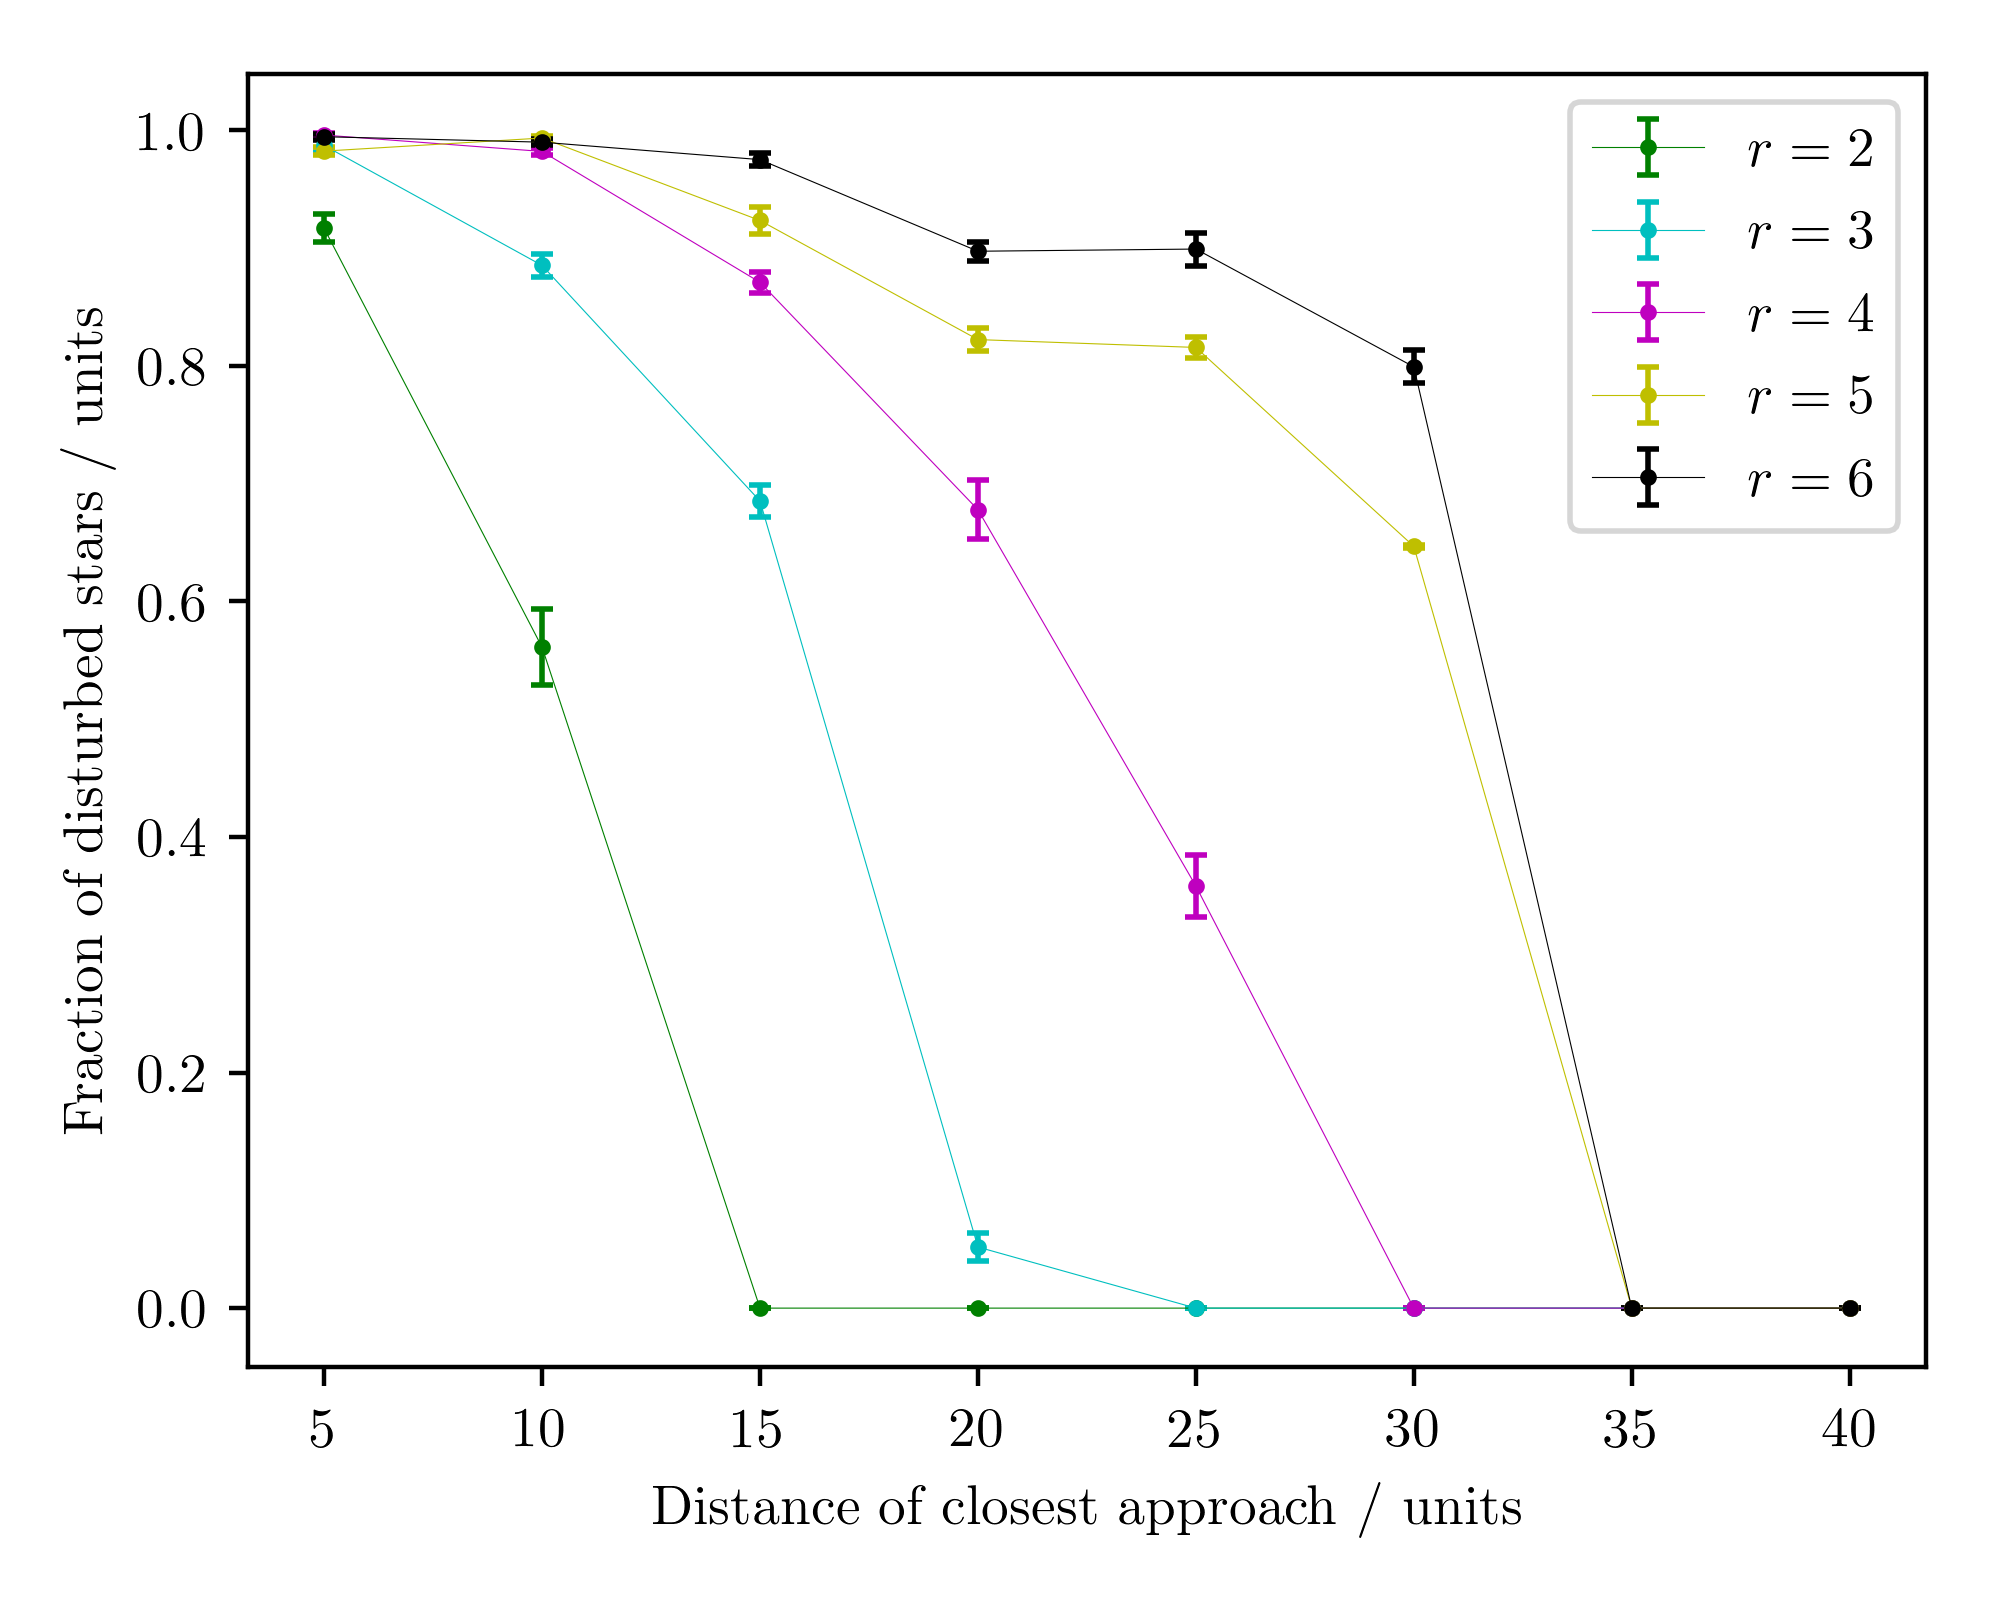
\includegraphics[width=\linewidth]{images/plot_fraction_rmin.png}
            \caption{Plots of the fraction of stars disturbed from their initial orbit against the mass of the perturbing galaxy (top plot) and the distance of closest approach (bottom plot) for each initial orbiting radius.}
            \label{figure:varying_fraction}
        \end{figure}

        \begin{figure}
            \centering
            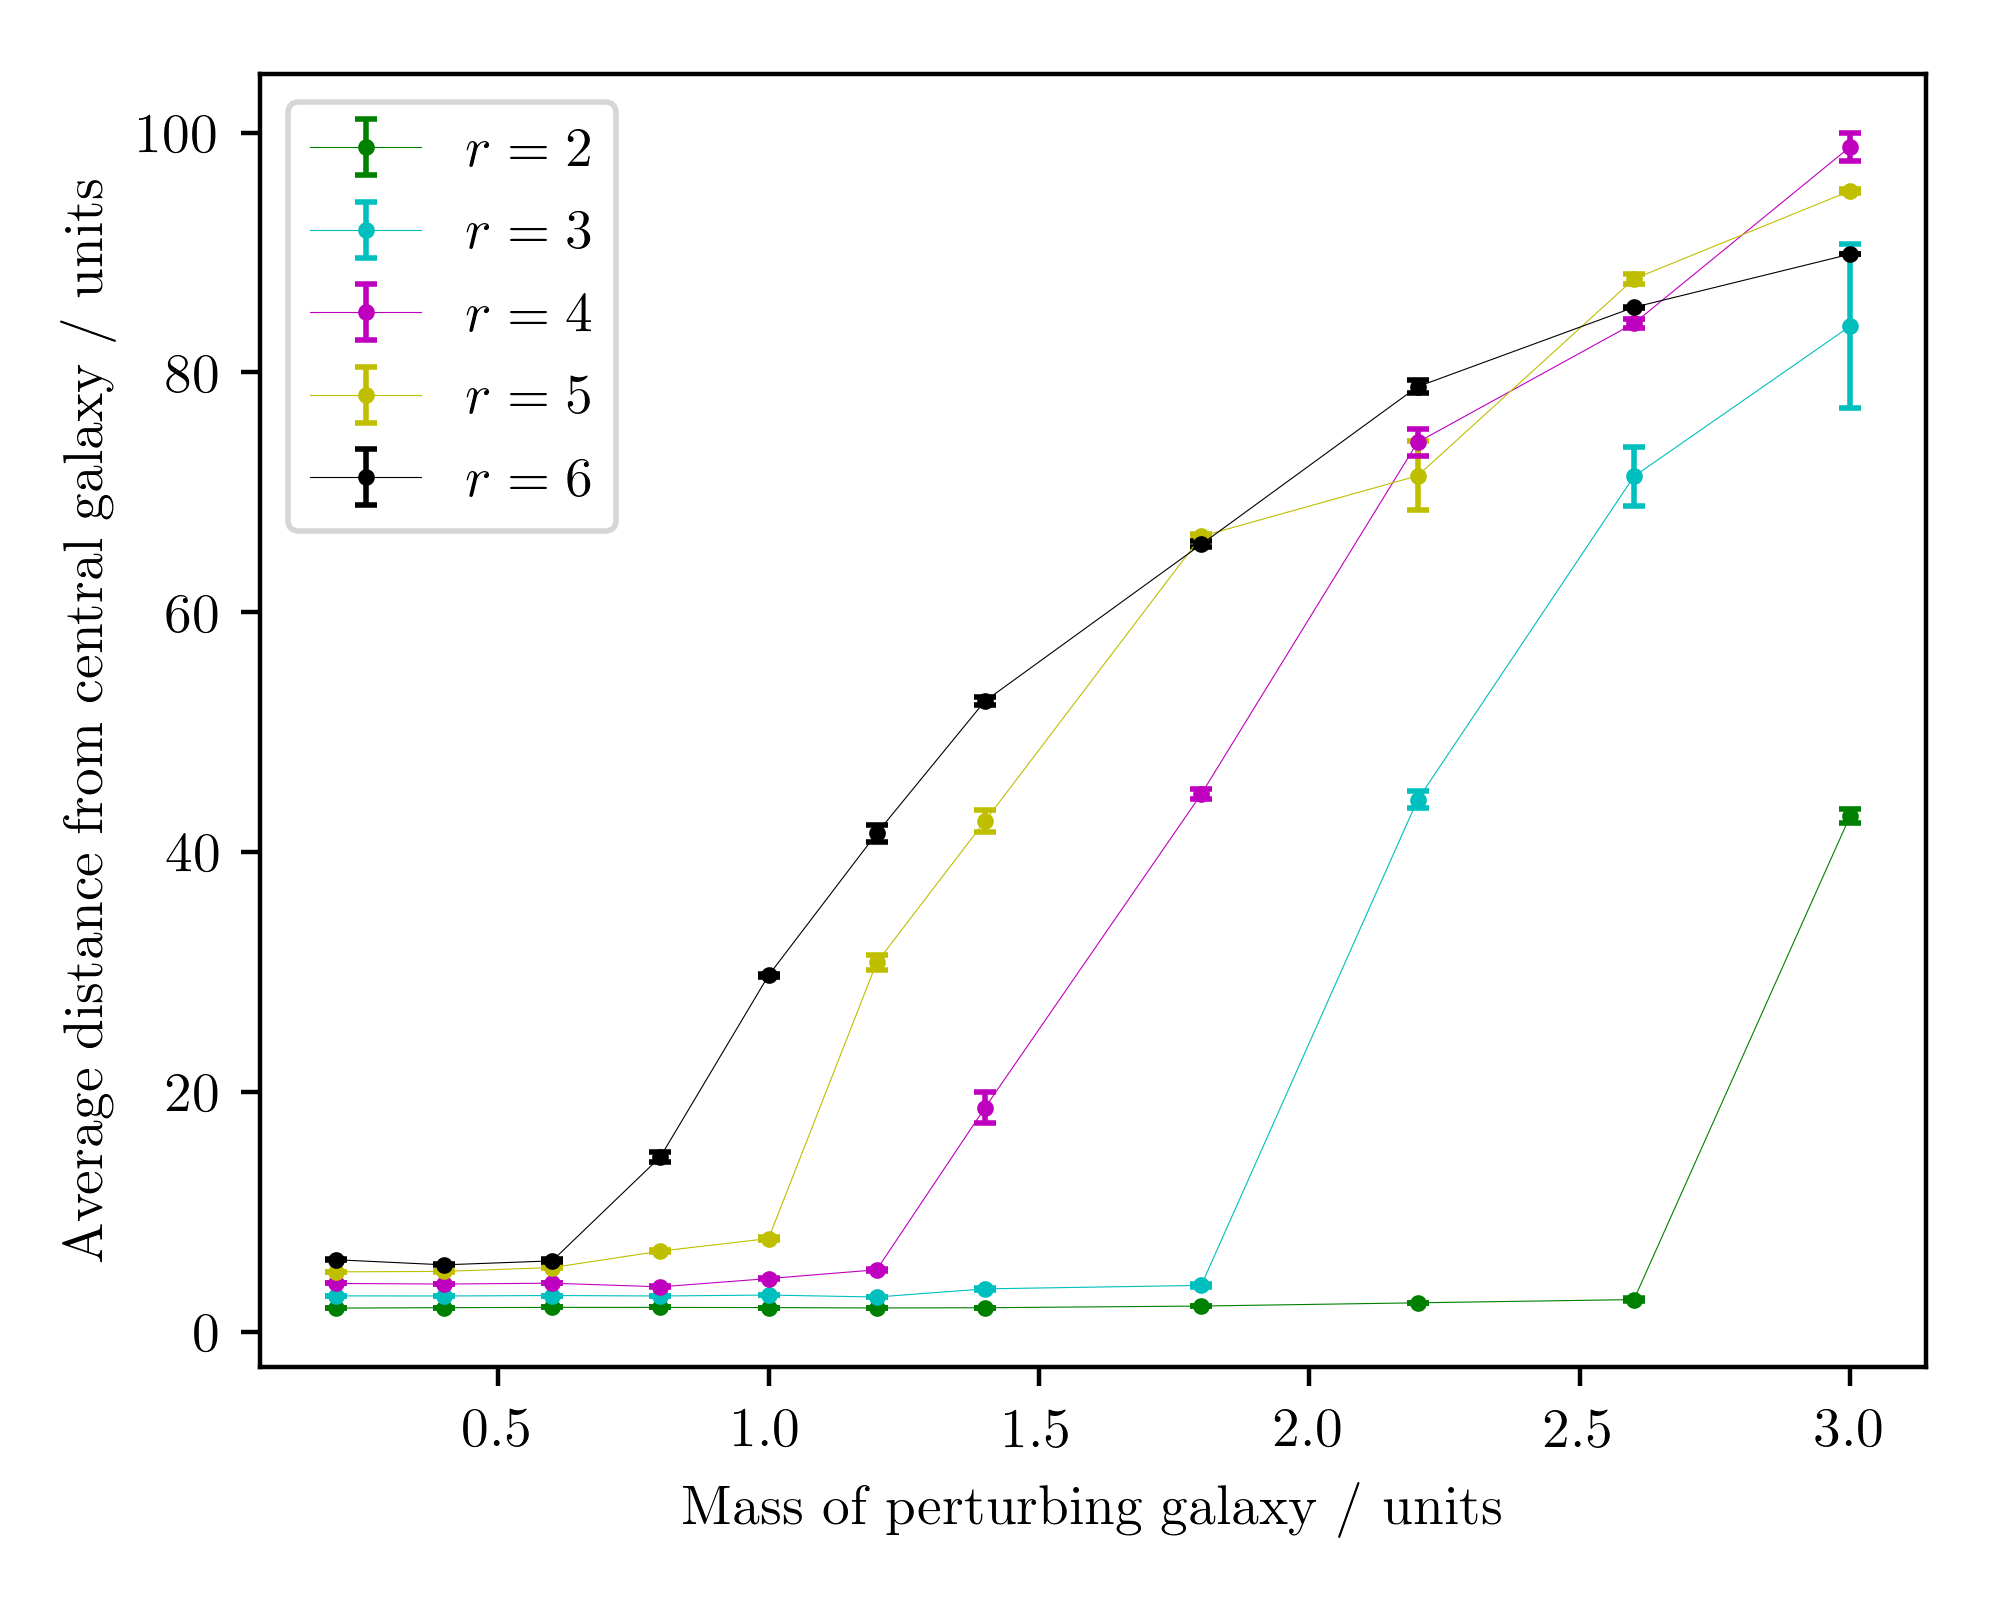
\includegraphics[width=\linewidth]{images/plot_distance_mass.png}
            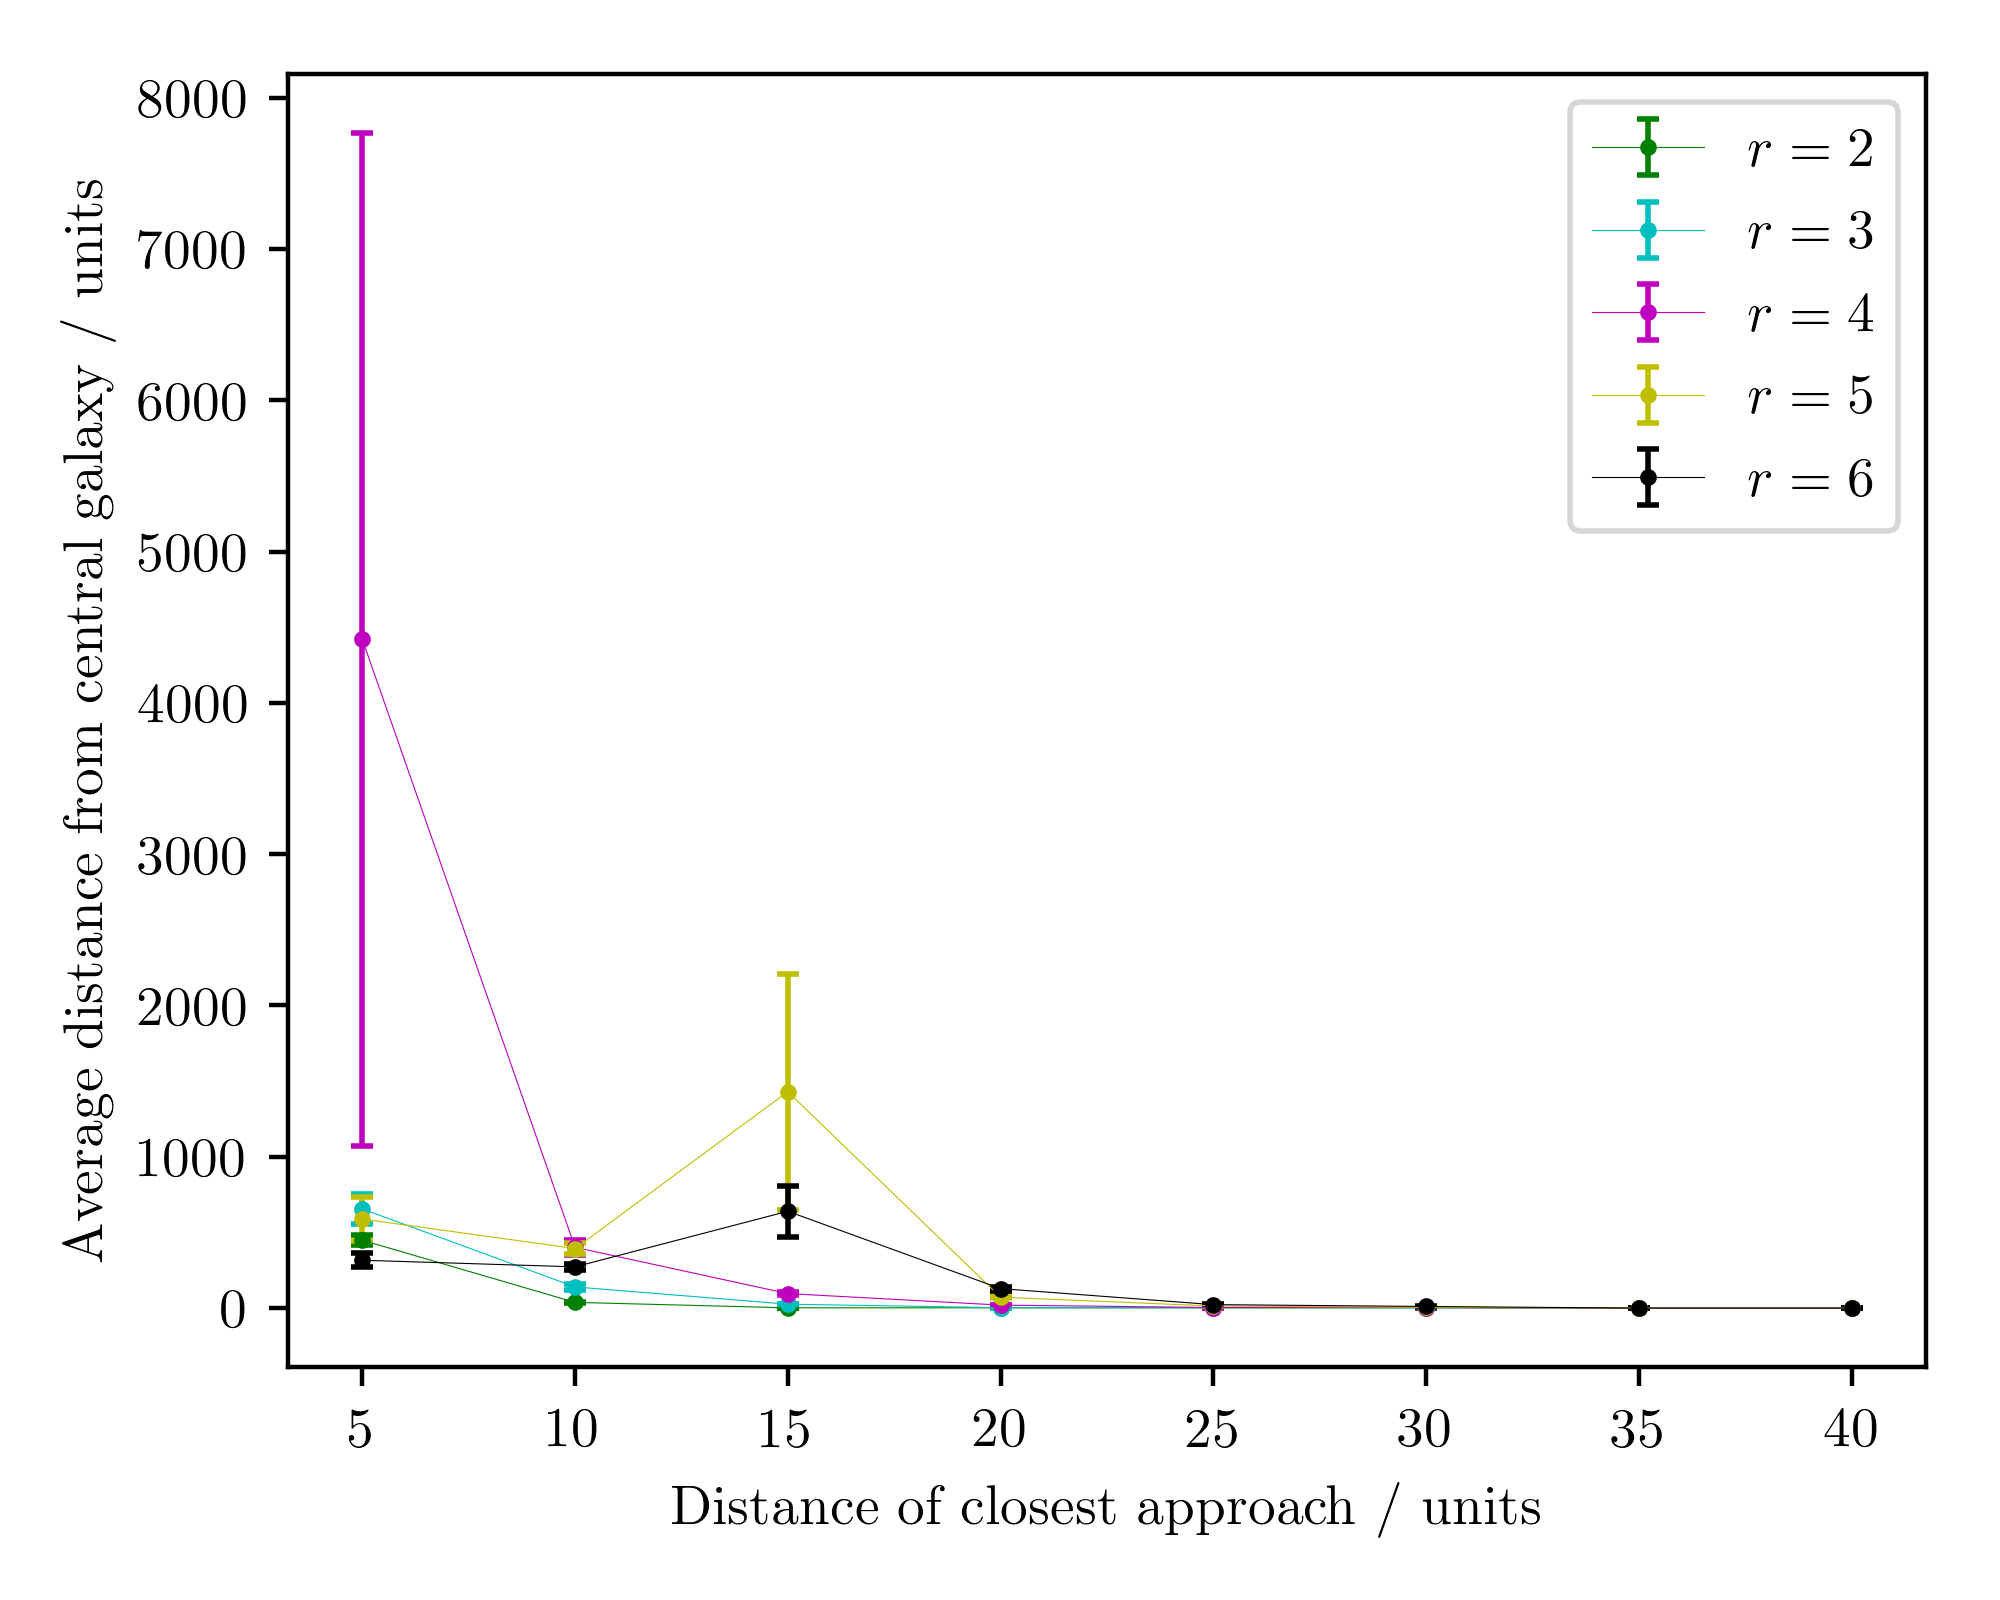
\includegraphics[width=\linewidth]{images/plot_distance_rmin.png}
            \caption{Plots of the median distance between the test particles and the central galaxy mass of the perturbing galaxy (top plot) and the distance of closest approach (bottom plot) for each initial orbiting radius.}
            \label{figure:varying_distance}
        \end{figure}

        As mentioned in \S \ref{section:implementation}, two quantitative metrics were used here -- the fraction of disturbed stars and the median distance between test particles and the central galaxy. These quantitative metrics were calculated at the snapshot $t = 100$ units after the frame where the distance between the two galaxies was at a minimum. The results of varying the mass of the perturbing galaxy and the distance of closest approach are shown in Figure \ref{figure:varying_fraction} and Figure \ref{figure:varying_distance}. Three independent runs of the simulation were performed for each data point, and the errors shown in the plots are the standard error of the mean from the three runs. 
        
        Both figures show general trends that are expected from intuition, where a more massive perturbing galaxy and/or a smaller distance of closest approach leads to a larger disruption of the orbiting stars. Both figures also show that stars with a larger orbiting radius are more easily disturbed, and this is most clearly seen in both plots in Figure \ref{figure:varying_fraction}, where the graph for $r = 5, 6$ has a high number of disturbed stars even at low perturbing mass and a large distance of closest approach. 
        
        Figure \ref{figure:varying_distance} shows how the median distance varies in the experiments. The top plot generally shows that stars at larger orbiting radius get flung out further as the mass of the perturbing galaxy increases. It also shows an interesting characteristic, where the median distance for different orbiting radii appear to converge at larger masses of the perturbing galaxy. However, further experimentation is required to provide a more concrete result. The bottom plot shows less conclusive results, where a smaller distance of approach does not necessarily mean stars with larger orbits can flung out further. However, the inconclusive results, large errors and absurdly large values here might be a product of the simulation setup, and this will be discussed in the following section \S \ref{section:error}.  
        
         
    \subsection{Sources of Errors}
        \label{section:error}

        From the results above, in particular for the median distance between the test particles and the central galaxy, there appears to be a large source of error. Looking into the setup of the simulation, this large error can be traced to the fact that the galaxies are treated as point masses. When a test particle gets very close ($r \to 0$) to the galaxies represented as point masses, the acceleration of the test particle, given as $a_{x} = GM(x - X) / r^3$, will become extremely large. This results in the test particle being 'shot' extremely far outwards, and this effect can actually be observed in the absurdly large error and distance in the bottom plot of Figure \ref{figure:varying_distance}. In order to mitigate this effect, the massive galaxies should be modelled to either have a finite radius or tweaking the potential such that the galaxies have a repulsive force at small radii. This was also the primary reason that the median rather than the average distance was used as the quantitative metric. 

        Another potential source of error in this simulation is the use of a finite timestep. It is impossible to achieve an infinitesimally small timestep due to the restrictions of a classical computer, however a sufficiently small finite timestep would create a reliable and accurate simulation. The choice of picking a timestep of \texttt{dt = 0.1} was a balance between the accuracy and the efficiency of the simulation. A larger timestep can lead to inaccuracies and can potentailly lead to a divergence of the positions and velocities of the simulated particles. A smaller timestep would mean a slower program, where given the timestep method is of order $\mathcal{O}(N^2)$, a decrease of the timestep by a factor of 10 would result in a runtime of 100 times longer, which is not ideal!

        A final, albeit minor, factor for the error of this simulation is the assumption that the test particles are collision-less. Collisions between stars can change the trajectories of the stars and potentially result in a different outcome to the simulation. The concept of viscosity in interstellar medium arises from such collisions, and this can lead to a different and/or more interesting fluid dynamical outcome. However, the scale of a galaxy is much bigger than that of a star, and such effects are often negligible in scenarios like this in the simulation. Thus, the assumption of collision-less test particles is a sound assumption in this simulation. 

\section{Conclusion}

        Using the simple timestep method, this simulation was able to successfully simulate the formation of tidal tails through the close encounter between two galaxies. This simulation was able to recreate parts of the results of the simulations performed by Toomre and Toomre in 1972, where prograde encounters were found to be significantly more disruptive than retrograde encounters. The strong tidal effects in prograde encounters were found to be the cause of the formation of tidal tails.

        In addition, experiments varying the mass of the perturbing galaxy and the distance of closest approach between the two galaxies showed intuitive results. These experiments showed that a heavier perturbing galaxy and/or a smaller distance of closest approach would result in a larger disruption caused by the perturbing galaxy. A larger proportion of stars were disturbed and displaced from their initial orbits, and the median distance between the test particles and the central galaxy was larger. Test particles with larger initial radius was also found to be more easily disturbed than those with a smaller initial radius.  

\vfill
        
\bibliography{report}{}
\bibliographystyle{unsrt}
    

\onecolumn
\section{Appendix}

{\large \texttt{core.py}}
\lstinputlisting{../core.py}
\newpage

\noindent {\large \texttt{simulation.py}}
\lstinputlisting{../simulation.py}
\newpage

\noindent {\large \texttt{animation.py}}
\lstinputlisting{../animation.py}
\newpage

\noindent {\large \texttt{get\_quantitative.py}}
\lstinputlisting{../get_quantitative.py}
\newpage


\end{document}
